\section{Genetic Algorithm}
\subsection{Description of the solution}
The genetic algorithms are currently well known so only the introduction of the presented solution is further done. Authors chose four parameters to be identified by the algorithm:

\begin{itemize}
	\item $D_X$... the distance between the pillars.
	\item $D_Y$... overlap of the lamp from the pillar axis. The positive values were considered in the direction getting closer to the sidewalk.
	\item $Z$... the pillar high.
	\item $\alpha$... the lamp tilt.
\end{itemize}

The DNA string was made in the order of appearance of each value. The same value limits were chosen for each tested lamp:

\begin{equation}
D_X \in \left\langle 0.5 \text{ m}, 50 \text{ m}\right\rangle
\end{equation}

\begin{equation}
D_Y \in \left\langle -2 \text{ m}, 2 \text{ m}\right\rangle
\end{equation}

\begin{equation}
Z \in \left\langle 2 \text{ m}, 15 \text{ m}\right\rangle
\end{equation}

\begin{equation}
\alpha \in \left\langle 0^\circ, 20^\circ \right\rangle
\end{equation}

The algorithm evaluated the illuminance at the sidewalk of length 200~m and width 3~m. The control area was set in the middle of the sidewalk of the length 80~m. Control area consisted of 6000 points evenly covering the whole field with 20~cm distances between each other. These points were used for illuminance evaluation. The pillars were placed 1~m out of the sidewalk. The pillars placement just shifted the overlap of the lamp. So the same effect could be done by setting the limits of DY in interval $\left\langle -3 \text{ m}, 1 \text{ m}\right\rangle$ with the pillars at the bound of the sidewalk.

\begin{figure}[htb]
  \centering
  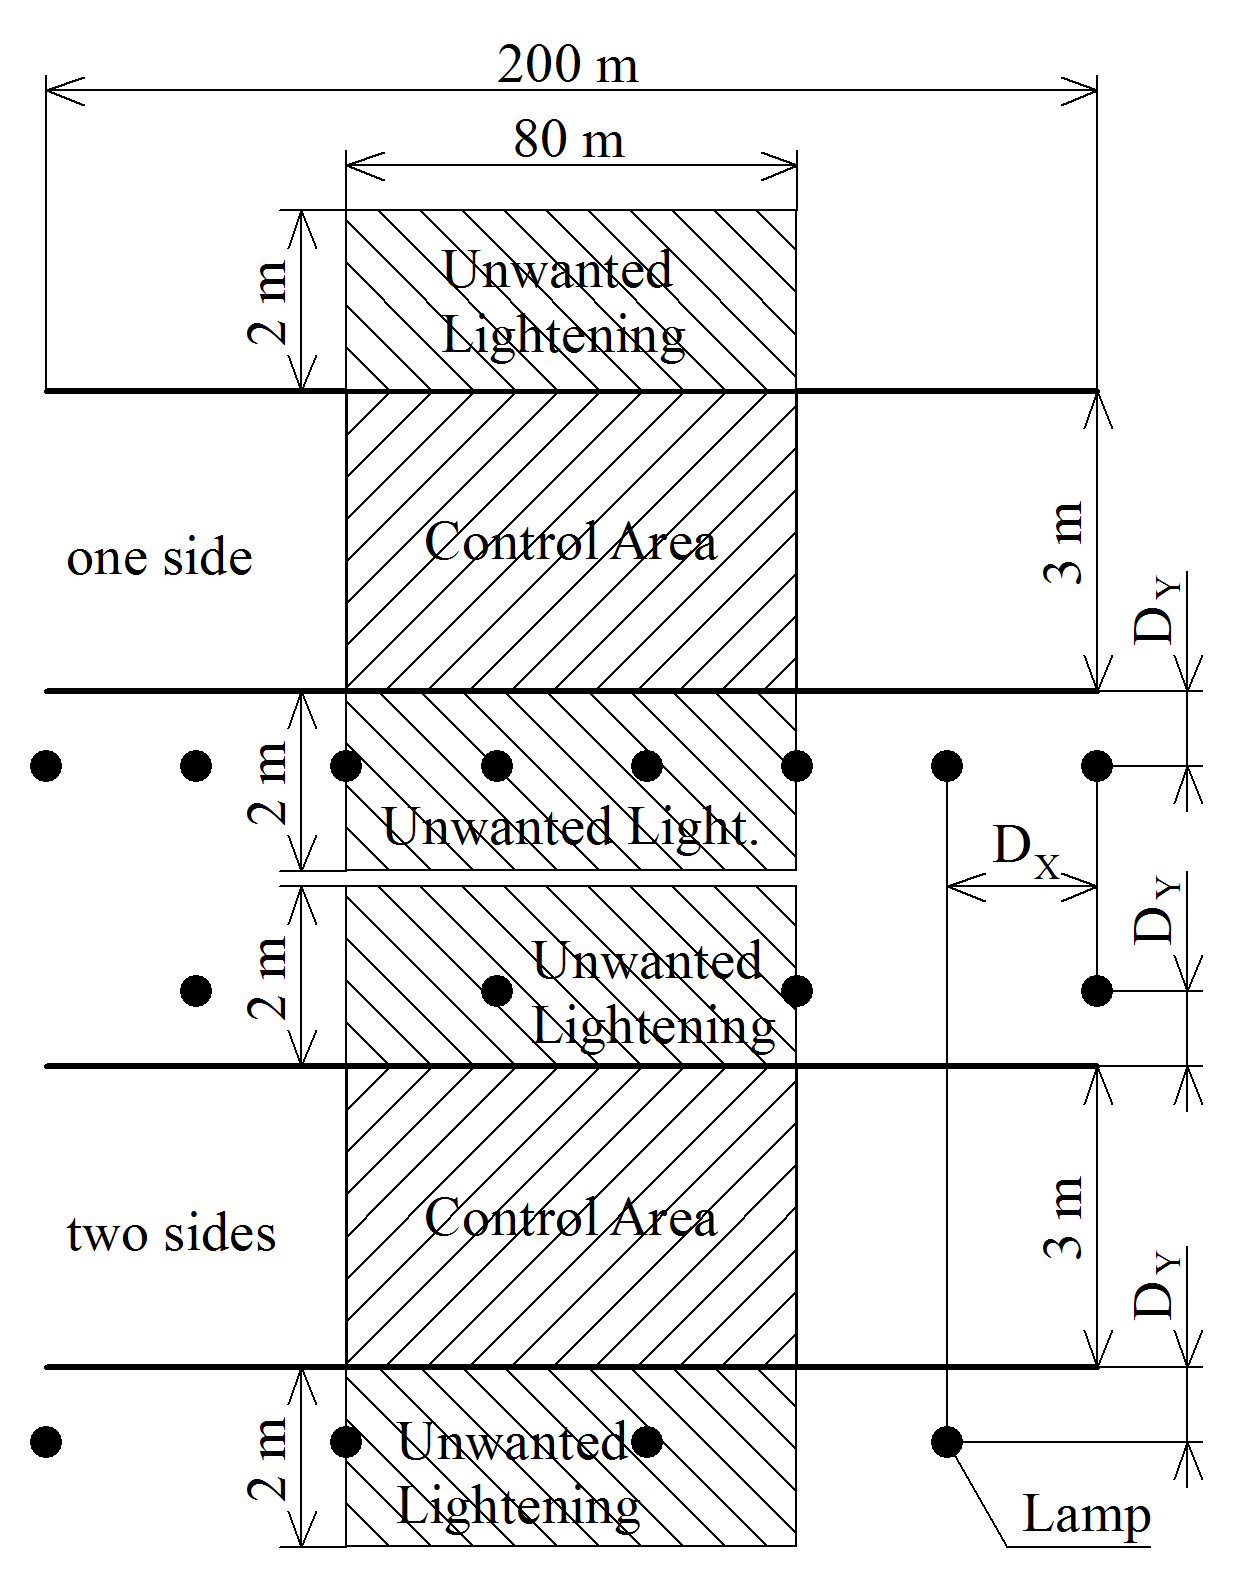
\includegraphics[width=0.8\columnwidth]{kotyChodniku}
  \caption{Dimensions of studied sidewalks}
  \label{fig:sidewalk}
\end{figure}

Two cases of of lamp placement was studied as it is shown in figure~\ref{fig:sidewalk}.

\subsection{Fitness function}
\subsection{Elitism}